% Options for packages loaded elsewhere
\PassOptionsToPackage{unicode}{hyperref}
\PassOptionsToPackage{hyphens}{url}
\PassOptionsToPackage{dvipsnames,svgnames,x11names}{xcolor}
%
\documentclass[
  letterpaper,
  DIV=11,
  numbers=noendperiod]{scrreprt}

\usepackage{amsmath,amssymb}
\usepackage{iftex}
\ifPDFTeX
  \usepackage[T1]{fontenc}
  \usepackage[utf8]{inputenc}
  \usepackage{textcomp} % provide euro and other symbols
\else % if luatex or xetex
  \usepackage{unicode-math}
  \defaultfontfeatures{Scale=MatchLowercase}
  \defaultfontfeatures[\rmfamily]{Ligatures=TeX,Scale=1}
\fi
\usepackage{lmodern}
\ifPDFTeX\else  
    % xetex/luatex font selection
\fi
% Use upquote if available, for straight quotes in verbatim environments
\IfFileExists{upquote.sty}{\usepackage{upquote}}{}
\IfFileExists{microtype.sty}{% use microtype if available
  \usepackage[]{microtype}
  \UseMicrotypeSet[protrusion]{basicmath} % disable protrusion for tt fonts
}{}
\makeatletter
\@ifundefined{KOMAClassName}{% if non-KOMA class
  \IfFileExists{parskip.sty}{%
    \usepackage{parskip}
  }{% else
    \setlength{\parindent}{0pt}
    \setlength{\parskip}{6pt plus 2pt minus 1pt}}
}{% if KOMA class
  \KOMAoptions{parskip=half}}
\makeatother
\usepackage{xcolor}
\setlength{\emergencystretch}{3em} % prevent overfull lines
\setcounter{secnumdepth}{5}
% Make \paragraph and \subparagraph free-standing
\ifx\paragraph\undefined\else
  \let\oldparagraph\paragraph
  \renewcommand{\paragraph}[1]{\oldparagraph{#1}\mbox{}}
\fi
\ifx\subparagraph\undefined\else
  \let\oldsubparagraph\subparagraph
  \renewcommand{\subparagraph}[1]{\oldsubparagraph{#1}\mbox{}}
\fi

\usepackage{color}
\usepackage{fancyvrb}
\newcommand{\VerbBar}{|}
\newcommand{\VERB}{\Verb[commandchars=\\\{\}]}
\DefineVerbatimEnvironment{Highlighting}{Verbatim}{commandchars=\\\{\}}
% Add ',fontsize=\small' for more characters per line
\usepackage{framed}
\definecolor{shadecolor}{RGB}{241,243,245}
\newenvironment{Shaded}{\begin{snugshade}}{\end{snugshade}}
\newcommand{\AlertTok}[1]{\textcolor[rgb]{0.68,0.00,0.00}{#1}}
\newcommand{\AnnotationTok}[1]{\textcolor[rgb]{0.37,0.37,0.37}{#1}}
\newcommand{\AttributeTok}[1]{\textcolor[rgb]{0.40,0.45,0.13}{#1}}
\newcommand{\BaseNTok}[1]{\textcolor[rgb]{0.68,0.00,0.00}{#1}}
\newcommand{\BuiltInTok}[1]{\textcolor[rgb]{0.00,0.23,0.31}{#1}}
\newcommand{\CharTok}[1]{\textcolor[rgb]{0.13,0.47,0.30}{#1}}
\newcommand{\CommentTok}[1]{\textcolor[rgb]{0.37,0.37,0.37}{#1}}
\newcommand{\CommentVarTok}[1]{\textcolor[rgb]{0.37,0.37,0.37}{\textit{#1}}}
\newcommand{\ConstantTok}[1]{\textcolor[rgb]{0.56,0.35,0.01}{#1}}
\newcommand{\ControlFlowTok}[1]{\textcolor[rgb]{0.00,0.23,0.31}{#1}}
\newcommand{\DataTypeTok}[1]{\textcolor[rgb]{0.68,0.00,0.00}{#1}}
\newcommand{\DecValTok}[1]{\textcolor[rgb]{0.68,0.00,0.00}{#1}}
\newcommand{\DocumentationTok}[1]{\textcolor[rgb]{0.37,0.37,0.37}{\textit{#1}}}
\newcommand{\ErrorTok}[1]{\textcolor[rgb]{0.68,0.00,0.00}{#1}}
\newcommand{\ExtensionTok}[1]{\textcolor[rgb]{0.00,0.23,0.31}{#1}}
\newcommand{\FloatTok}[1]{\textcolor[rgb]{0.68,0.00,0.00}{#1}}
\newcommand{\FunctionTok}[1]{\textcolor[rgb]{0.28,0.35,0.67}{#1}}
\newcommand{\ImportTok}[1]{\textcolor[rgb]{0.00,0.46,0.62}{#1}}
\newcommand{\InformationTok}[1]{\textcolor[rgb]{0.37,0.37,0.37}{#1}}
\newcommand{\KeywordTok}[1]{\textcolor[rgb]{0.00,0.23,0.31}{#1}}
\newcommand{\NormalTok}[1]{\textcolor[rgb]{0.00,0.23,0.31}{#1}}
\newcommand{\OperatorTok}[1]{\textcolor[rgb]{0.37,0.37,0.37}{#1}}
\newcommand{\OtherTok}[1]{\textcolor[rgb]{0.00,0.23,0.31}{#1}}
\newcommand{\PreprocessorTok}[1]{\textcolor[rgb]{0.68,0.00,0.00}{#1}}
\newcommand{\RegionMarkerTok}[1]{\textcolor[rgb]{0.00,0.23,0.31}{#1}}
\newcommand{\SpecialCharTok}[1]{\textcolor[rgb]{0.37,0.37,0.37}{#1}}
\newcommand{\SpecialStringTok}[1]{\textcolor[rgb]{0.13,0.47,0.30}{#1}}
\newcommand{\StringTok}[1]{\textcolor[rgb]{0.13,0.47,0.30}{#1}}
\newcommand{\VariableTok}[1]{\textcolor[rgb]{0.07,0.07,0.07}{#1}}
\newcommand{\VerbatimStringTok}[1]{\textcolor[rgb]{0.13,0.47,0.30}{#1}}
\newcommand{\WarningTok}[1]{\textcolor[rgb]{0.37,0.37,0.37}{\textit{#1}}}

\providecommand{\tightlist}{%
  \setlength{\itemsep}{0pt}\setlength{\parskip}{0pt}}\usepackage{longtable,booktabs,array}
\usepackage{calc} % for calculating minipage widths
% Correct order of tables after \paragraph or \subparagraph
\usepackage{etoolbox}
\makeatletter
\patchcmd\longtable{\par}{\if@noskipsec\mbox{}\fi\par}{}{}
\makeatother
% Allow footnotes in longtable head/foot
\IfFileExists{footnotehyper.sty}{\usepackage{footnotehyper}}{\usepackage{footnote}}
\makesavenoteenv{longtable}
\usepackage{graphicx}
\makeatletter
\def\maxwidth{\ifdim\Gin@nat@width>\linewidth\linewidth\else\Gin@nat@width\fi}
\def\maxheight{\ifdim\Gin@nat@height>\textheight\textheight\else\Gin@nat@height\fi}
\makeatother
% Scale images if necessary, so that they will not overflow the page
% margins by default, and it is still possible to overwrite the defaults
% using explicit options in \includegraphics[width, height, ...]{}
\setkeys{Gin}{width=\maxwidth,height=\maxheight,keepaspectratio}
% Set default figure placement to htbp
\makeatletter
\def\fps@figure{htbp}
\makeatother
\newlength{\cslhangindent}
\setlength{\cslhangindent}{1.5em}
\newlength{\csllabelwidth}
\setlength{\csllabelwidth}{3em}
\newlength{\cslentryspacingunit} % times entry-spacing
\setlength{\cslentryspacingunit}{\parskip}
\newenvironment{CSLReferences}[2] % #1 hanging-ident, #2 entry spacing
 {% don't indent paragraphs
  \setlength{\parindent}{0pt}
  % turn on hanging indent if param 1 is 1
  \ifodd #1
  \let\oldpar\par
  \def\par{\hangindent=\cslhangindent\oldpar}
  \fi
  % set entry spacing
  \setlength{\parskip}{#2\cslentryspacingunit}
 }%
 {}
\usepackage{calc}
\newcommand{\CSLBlock}[1]{#1\hfill\break}
\newcommand{\CSLLeftMargin}[1]{\parbox[t]{\csllabelwidth}{#1}}
\newcommand{\CSLRightInline}[1]{\parbox[t]{\linewidth - \csllabelwidth}{#1}\break}
\newcommand{\CSLIndent}[1]{\hspace{\cslhangindent}#1}

\KOMAoption{captions}{tableheading}
\makeatletter
\makeatother
\makeatletter
\@ifpackageloaded{bookmark}{}{\usepackage{bookmark}}
\makeatother
\makeatletter
\@ifpackageloaded{caption}{}{\usepackage{caption}}
\AtBeginDocument{%
\ifdefined\contentsname
  \renewcommand*\contentsname{Table of contents}
\else
  \newcommand\contentsname{Table of contents}
\fi
\ifdefined\listfigurename
  \renewcommand*\listfigurename{List of Figures}
\else
  \newcommand\listfigurename{List of Figures}
\fi
\ifdefined\listtablename
  \renewcommand*\listtablename{List of Tables}
\else
  \newcommand\listtablename{List of Tables}
\fi
\ifdefined\figurename
  \renewcommand*\figurename{Figure}
\else
  \newcommand\figurename{Figure}
\fi
\ifdefined\tablename
  \renewcommand*\tablename{Table}
\else
  \newcommand\tablename{Table}
\fi
}
\@ifpackageloaded{float}{}{\usepackage{float}}
\floatstyle{ruled}
\@ifundefined{c@chapter}{\newfloat{codelisting}{h}{lop}}{\newfloat{codelisting}{h}{lop}[chapter]}
\floatname{codelisting}{Listing}
\newcommand*\listoflistings{\listof{codelisting}{List of Listings}}
\makeatother
\makeatletter
\@ifpackageloaded{caption}{}{\usepackage{caption}}
\@ifpackageloaded{subcaption}{}{\usepackage{subcaption}}
\makeatother
\makeatletter
\@ifpackageloaded{tcolorbox}{}{\usepackage[skins,breakable]{tcolorbox}}
\makeatother
\makeatletter
\@ifundefined{shadecolor}{\definecolor{shadecolor}{rgb}{.97, .97, .97}}
\makeatother
\makeatletter
\makeatother
\makeatletter
\makeatother
\ifLuaTeX
  \usepackage{selnolig}  % disable illegal ligatures
\fi
\IfFileExists{bookmark.sty}{\usepackage{bookmark}}{\usepackage{hyperref}}
\IfFileExists{xurl.sty}{\usepackage{xurl}}{} % add URL line breaks if available
\urlstyle{same} % disable monospaced font for URLs
\hypersetup{
  pdftitle={Introduction},
  pdfauthor={Nooriza Maharani},
  colorlinks=true,
  linkcolor={blue},
  filecolor={Maroon},
  citecolor={Blue},
  urlcolor={Blue},
  pdfcreator={LaTeX via pandoc}}

\title{Introduction}
\author{Nooriza Maharani}
\date{January 21, 2025}

\begin{document}
\maketitle
\ifdefined\Shaded\renewenvironment{Shaded}{\begin{tcolorbox}[borderline west={3pt}{0pt}{shadecolor}, frame hidden, boxrule=0pt, interior hidden, enhanced, sharp corners, breakable]}{\end{tcolorbox}}\fi

\renewcommand*\contentsname{Table of contents}
{
\hypersetup{linkcolor=}
\setcounter{tocdepth}{2}
\tableofcontents
}
\bookmarksetup{startatroot}

\hypertarget{rs-learning-diary}{%
\chapter{RS Learning Diary}\label{rs-learning-diary}}

This is a Quarto book to document my learning journey in \textbf{Remote
Sensing Cities and Environments} course during my time at CASA UCL
24/25, offering insights learned, its applications, and my own
reflections. The module is based on Dr Andrew Maclachlan github page
{[}\href{https://andrewmaclachlan.github.io/CASA0023/.}{here}{]}.

*For those of you who also want to learn Geographic Information Scicene
beyond `typical GIS' Software, as in use R-Studio, you could also visit
his other github page
{[}\href{https://andrewmaclachlan.github.io/CASA0005repo/index.html}{here}{]}.

\begin{center}\rule{0.5\linewidth}{0.5pt}\end{center}

\hypertarget{introduction}{%
\section{Introduction}\label{introduction}}

Hi, I'm Nooriza, a student currently pursuing a Master's degree in Urban
Spatial Science at UCL. I have an academic background in Geography with
a specialization in Regional Development Studies and have several
substantial work experience in government consultancies in Indonesia.

\hypertarget{why-do-i-choose-this-module}{%
\section{Why do I choose this
module?}\label{why-do-i-choose-this-module}}

The reason I take Remote Sensing course is my desire to know \emph{how
it feels to be a bird, seeing things from above, and to see the unseen.}
Don't we agree that remote sensing offers perspectives far beyond what
our human eyes can naturally perceive?

\begin{figure}

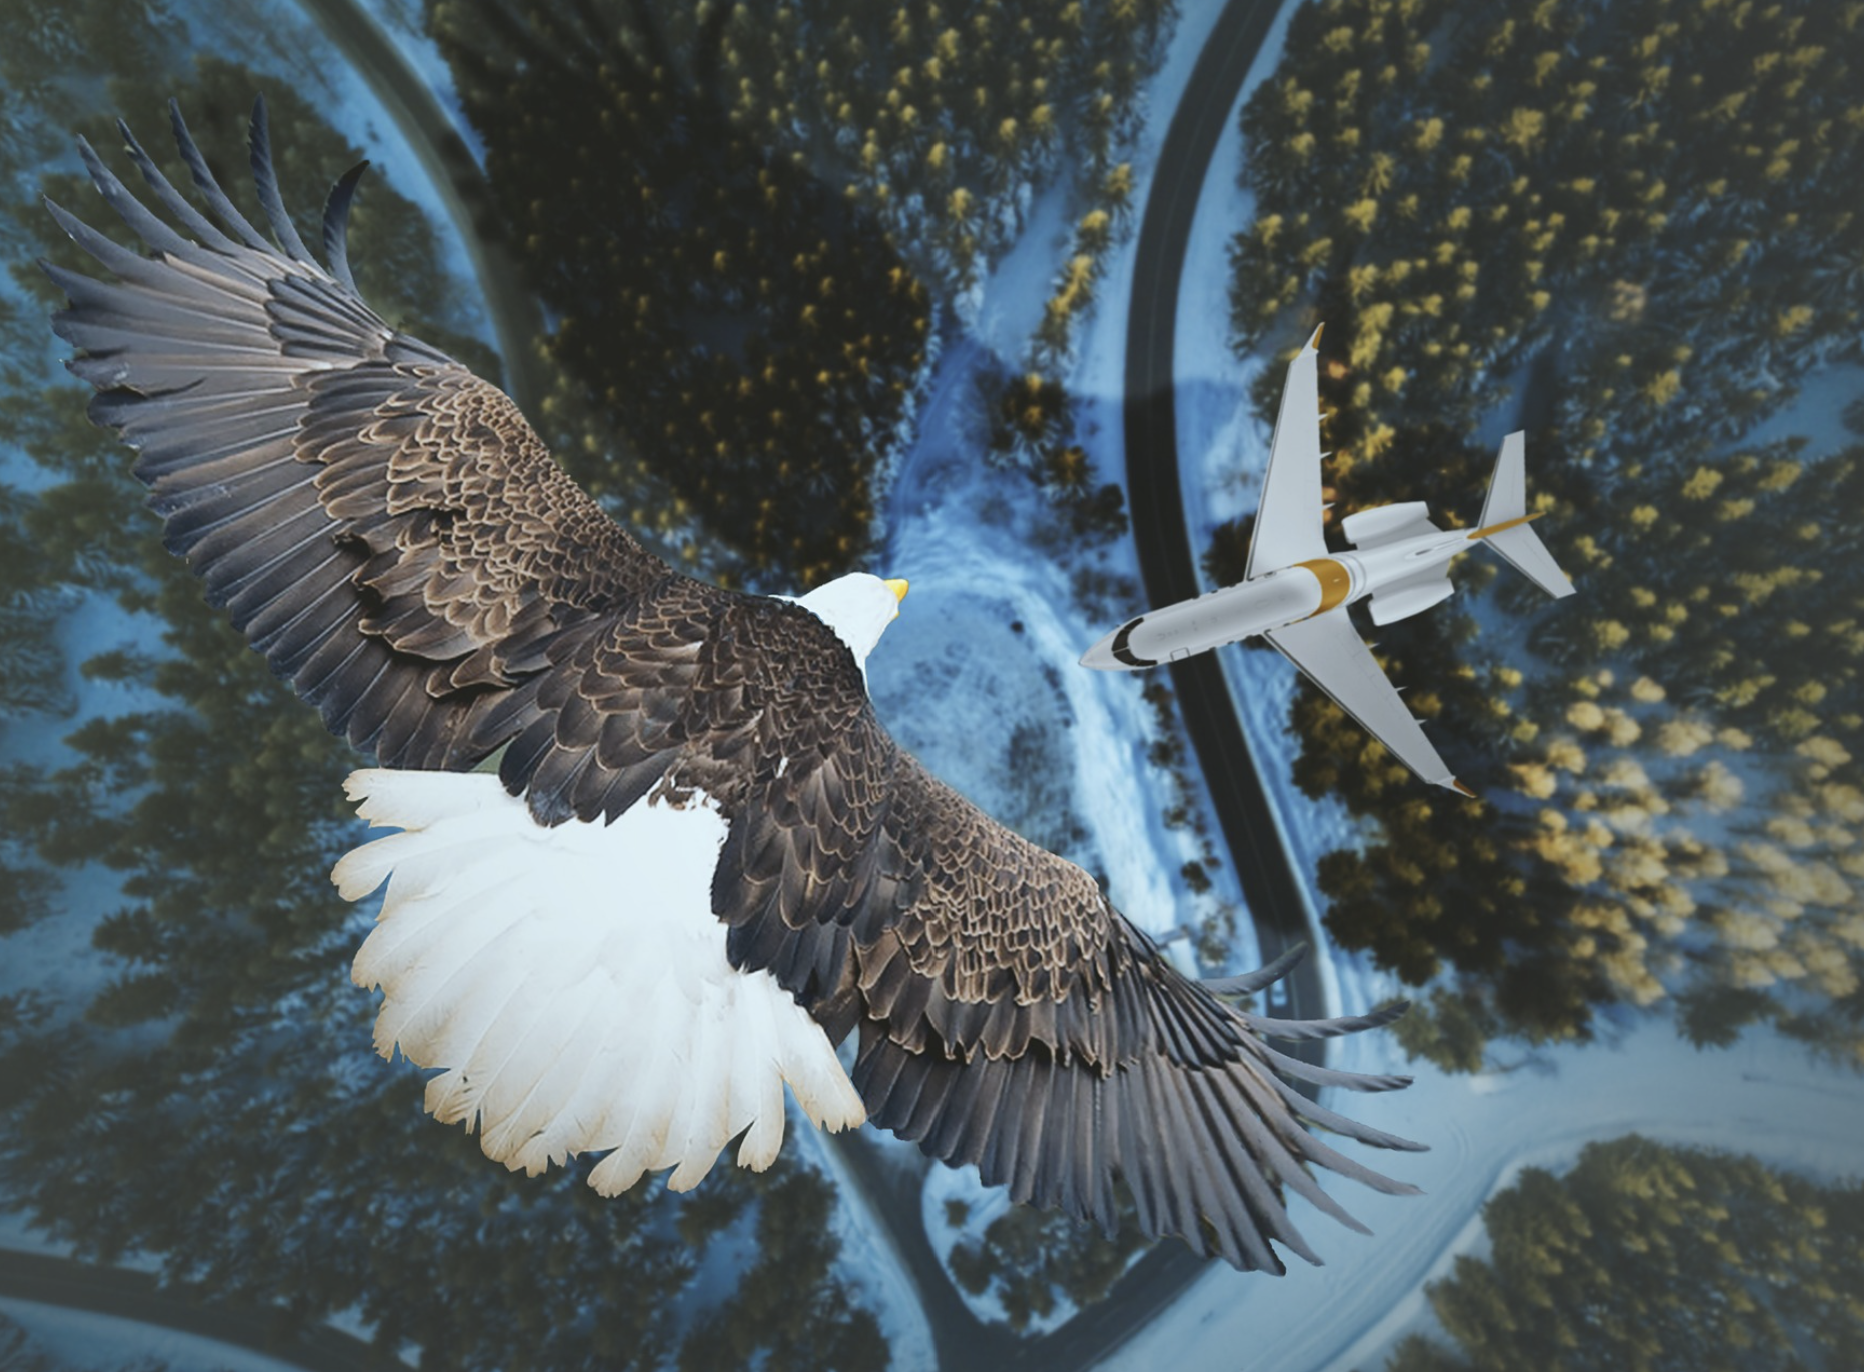
\includegraphics[width=5.07292in,height=\textheight]{images/clipboard-2217286199.png} \hfill{}

\end{figure}

source :
\href{https://chirpforbirds.com/nature-advocacy/biomimicry-and-birds/}{Biomimicry
and Birds}

\begin{figure}

\href{https://photojournal.jpl.nasa.gov/jpegMod/PIA02605_modest.jpg}{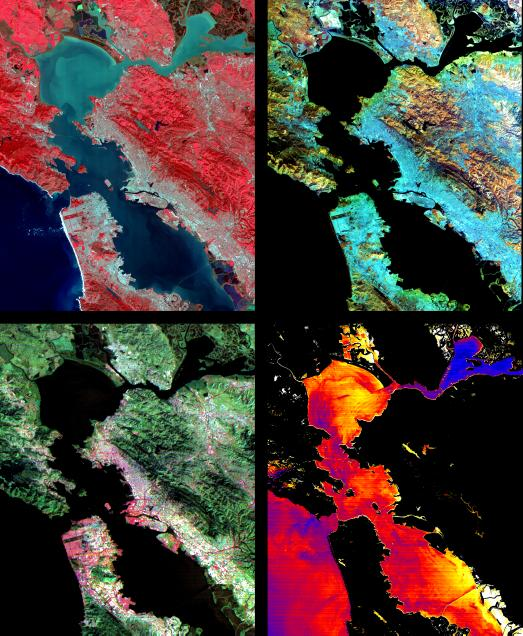
\includegraphics{images/PIA02605_modest.jpg}}

\end{figure}

source :
\href{https://photojournal.jpl.nasa.gov/catalog/PIA02605}{NASA/JPL}

For example the ASTER images of San Fransisco Bay above, it highlights
different object such as vegetation (upper left); soil \& rocks in
mountainous area (upper right); urban materials (lower left) ; and water
temperature (lower right).

Meanwhile, practically, learning this course will, hopefully, help me
address the challenges I faced during my previous work in Indonesia. For
example, while working on a project focused on healthcare accessibility
across hundreds of small islands, we struggled to obtain real-time data
to identify which islands were inhabited and which were not.
Additionally, we faced challenges in determining which islands had ports
suitable for docking ships. I believe that applying remote sensing data
is both cost- and time-efficient in helping the government maintain more
precise and up-to-date data, which is particularly important in world's
largest archipelago country like Indonesia.

Feel free to explore my site to learn more about my learning experience.
Hope it helps!

\bookmarksetup{startatroot}

\hypertarget{getting-to-know-remote-sensing}{%
\chapter{Getting to Know Remote
Sensing}\label{getting-to-know-remote-sensing}}

\hypertarget{summary}{%
\section{\texorpdfstring{\textbf{Summary}}{Summary}}\label{summary}}

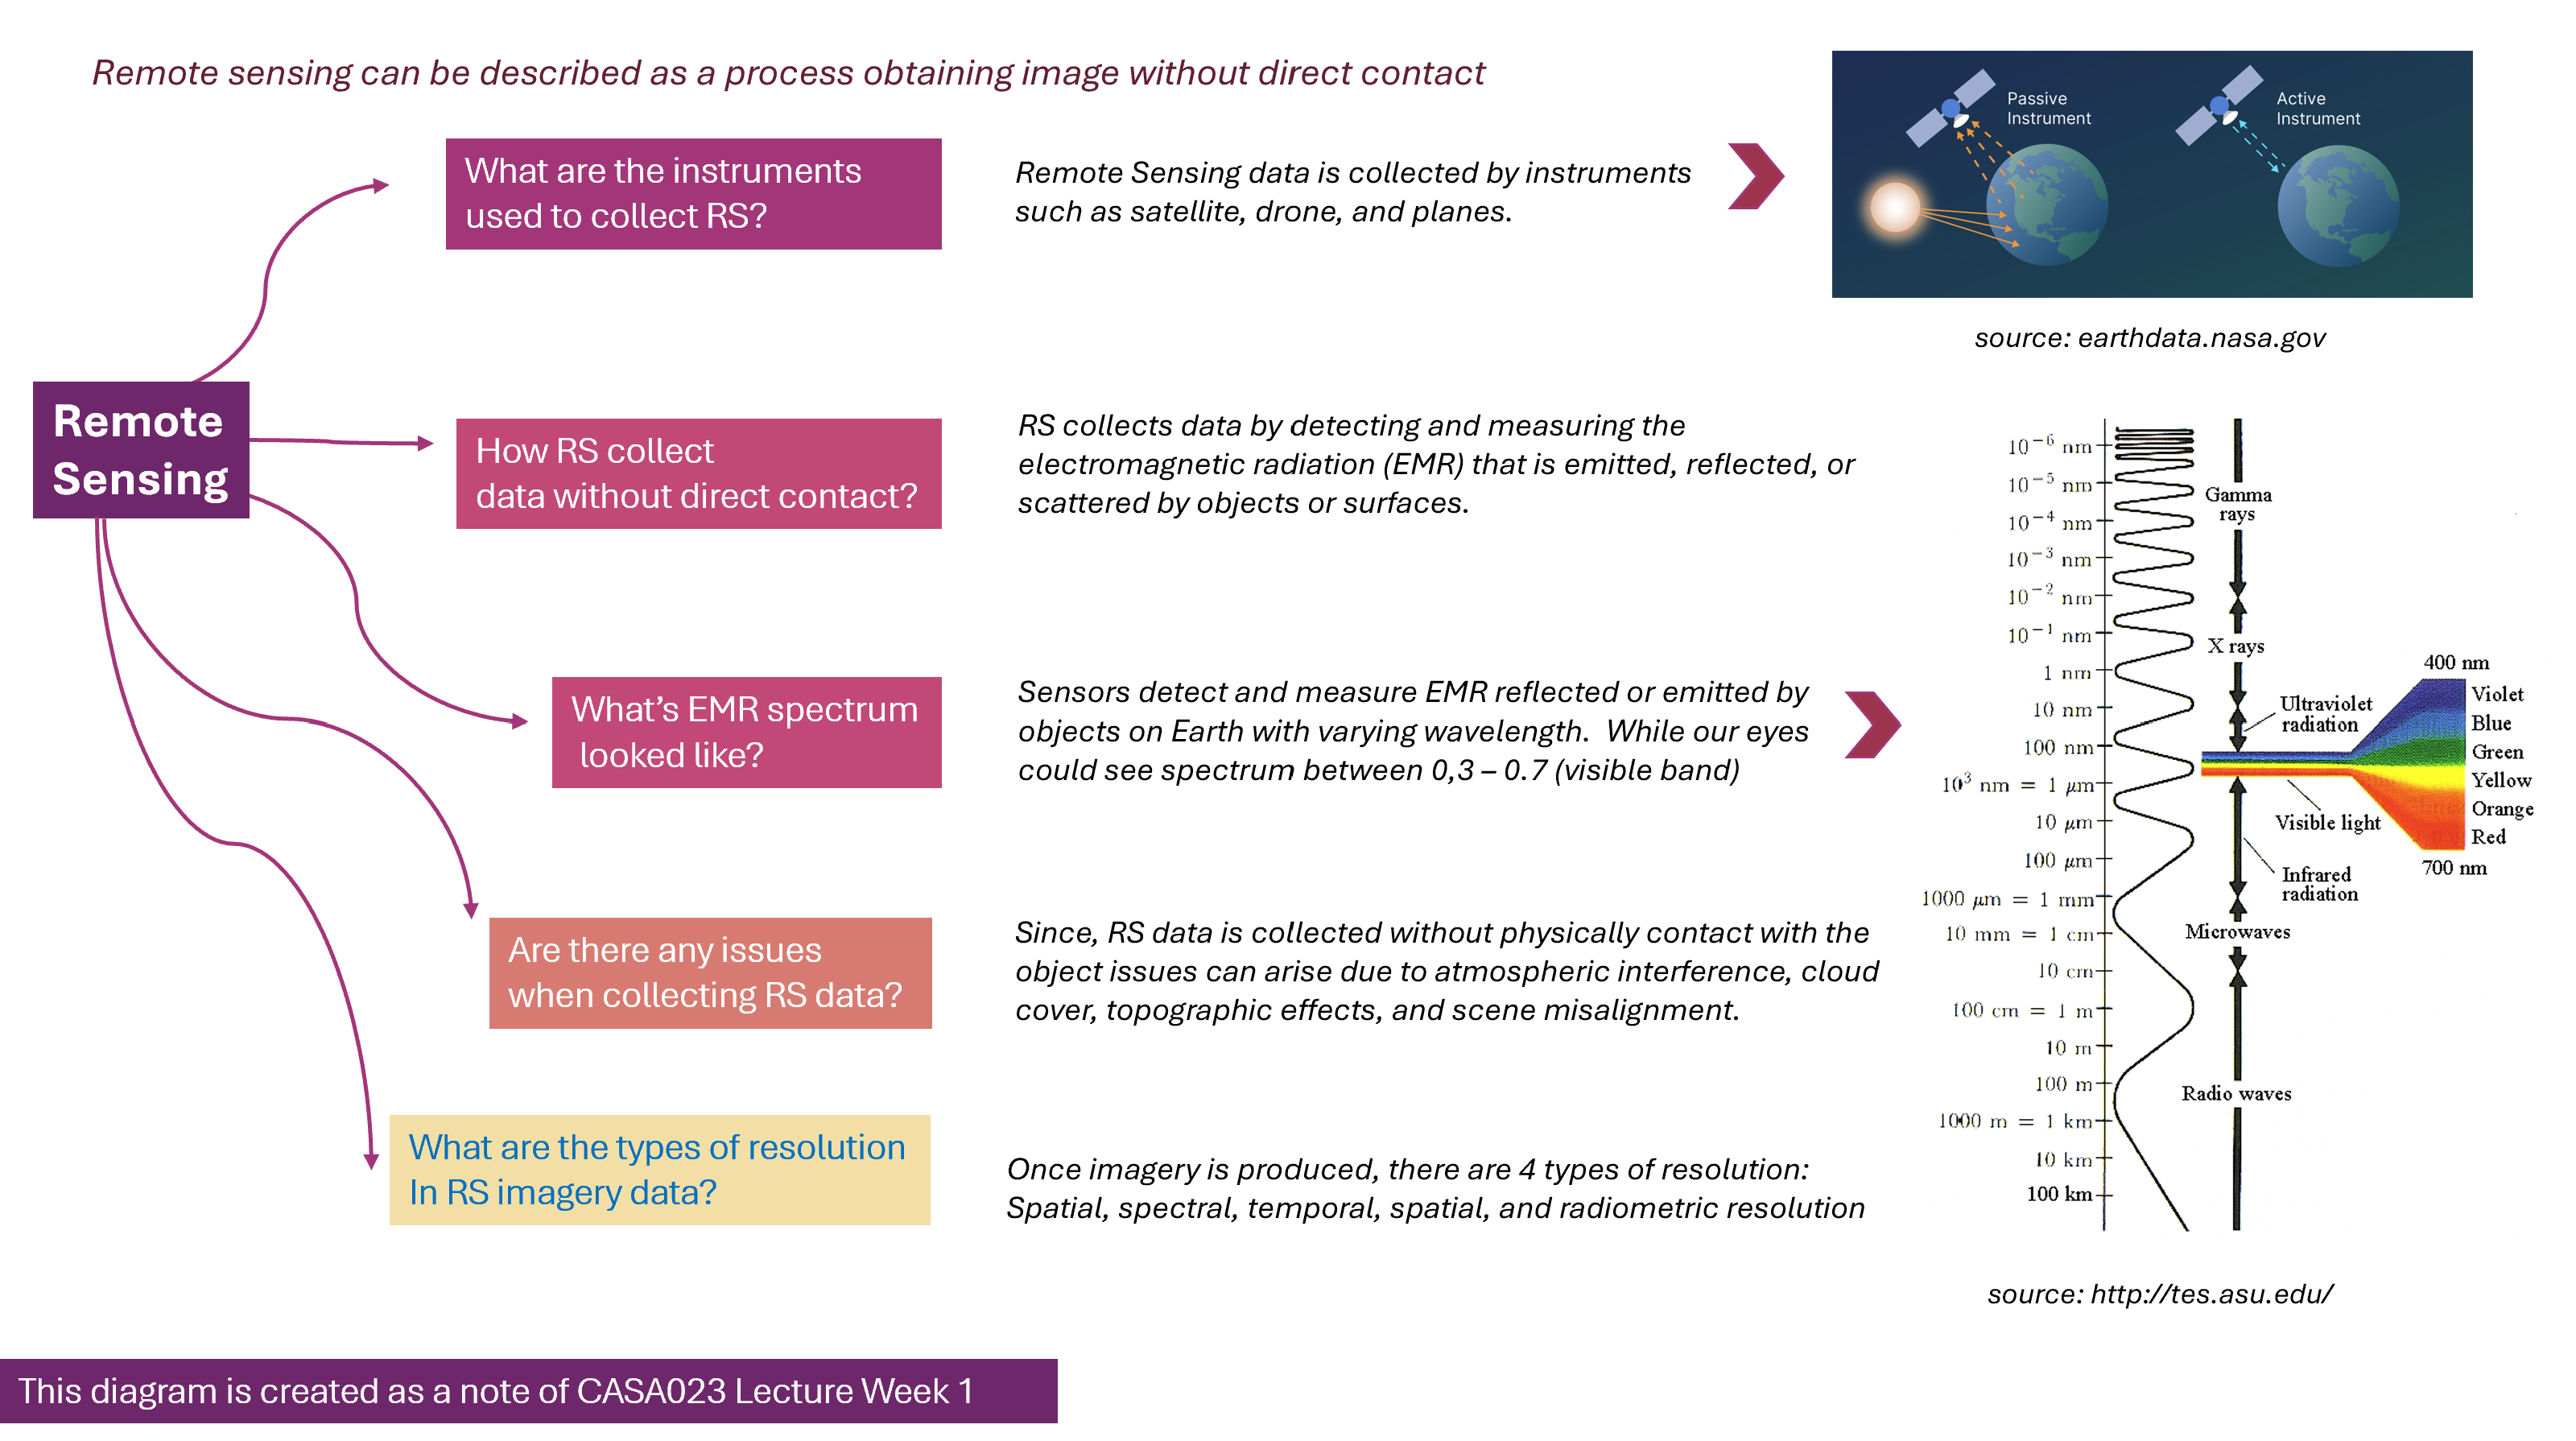
\includegraphics{images/clipboard-1084697230.png}

Meanwhile, this week practical is introducing 2 sources of imagery :

\begin{enumerate}
\def\labelenumi{\arabic{enumi}.}
\item
  a. Landsat-8

  The Landsat 8 satellite has a 16-day revisit cycle, meaning it can
  capture imagery of the same location every 16 day. This period would
  be advantageous to monitor changes at moderate pace, as its revisit
  time is every 16 days.
\end{enumerate}

\begin{itemize}
\item
  \begin{figure}

  {\centering 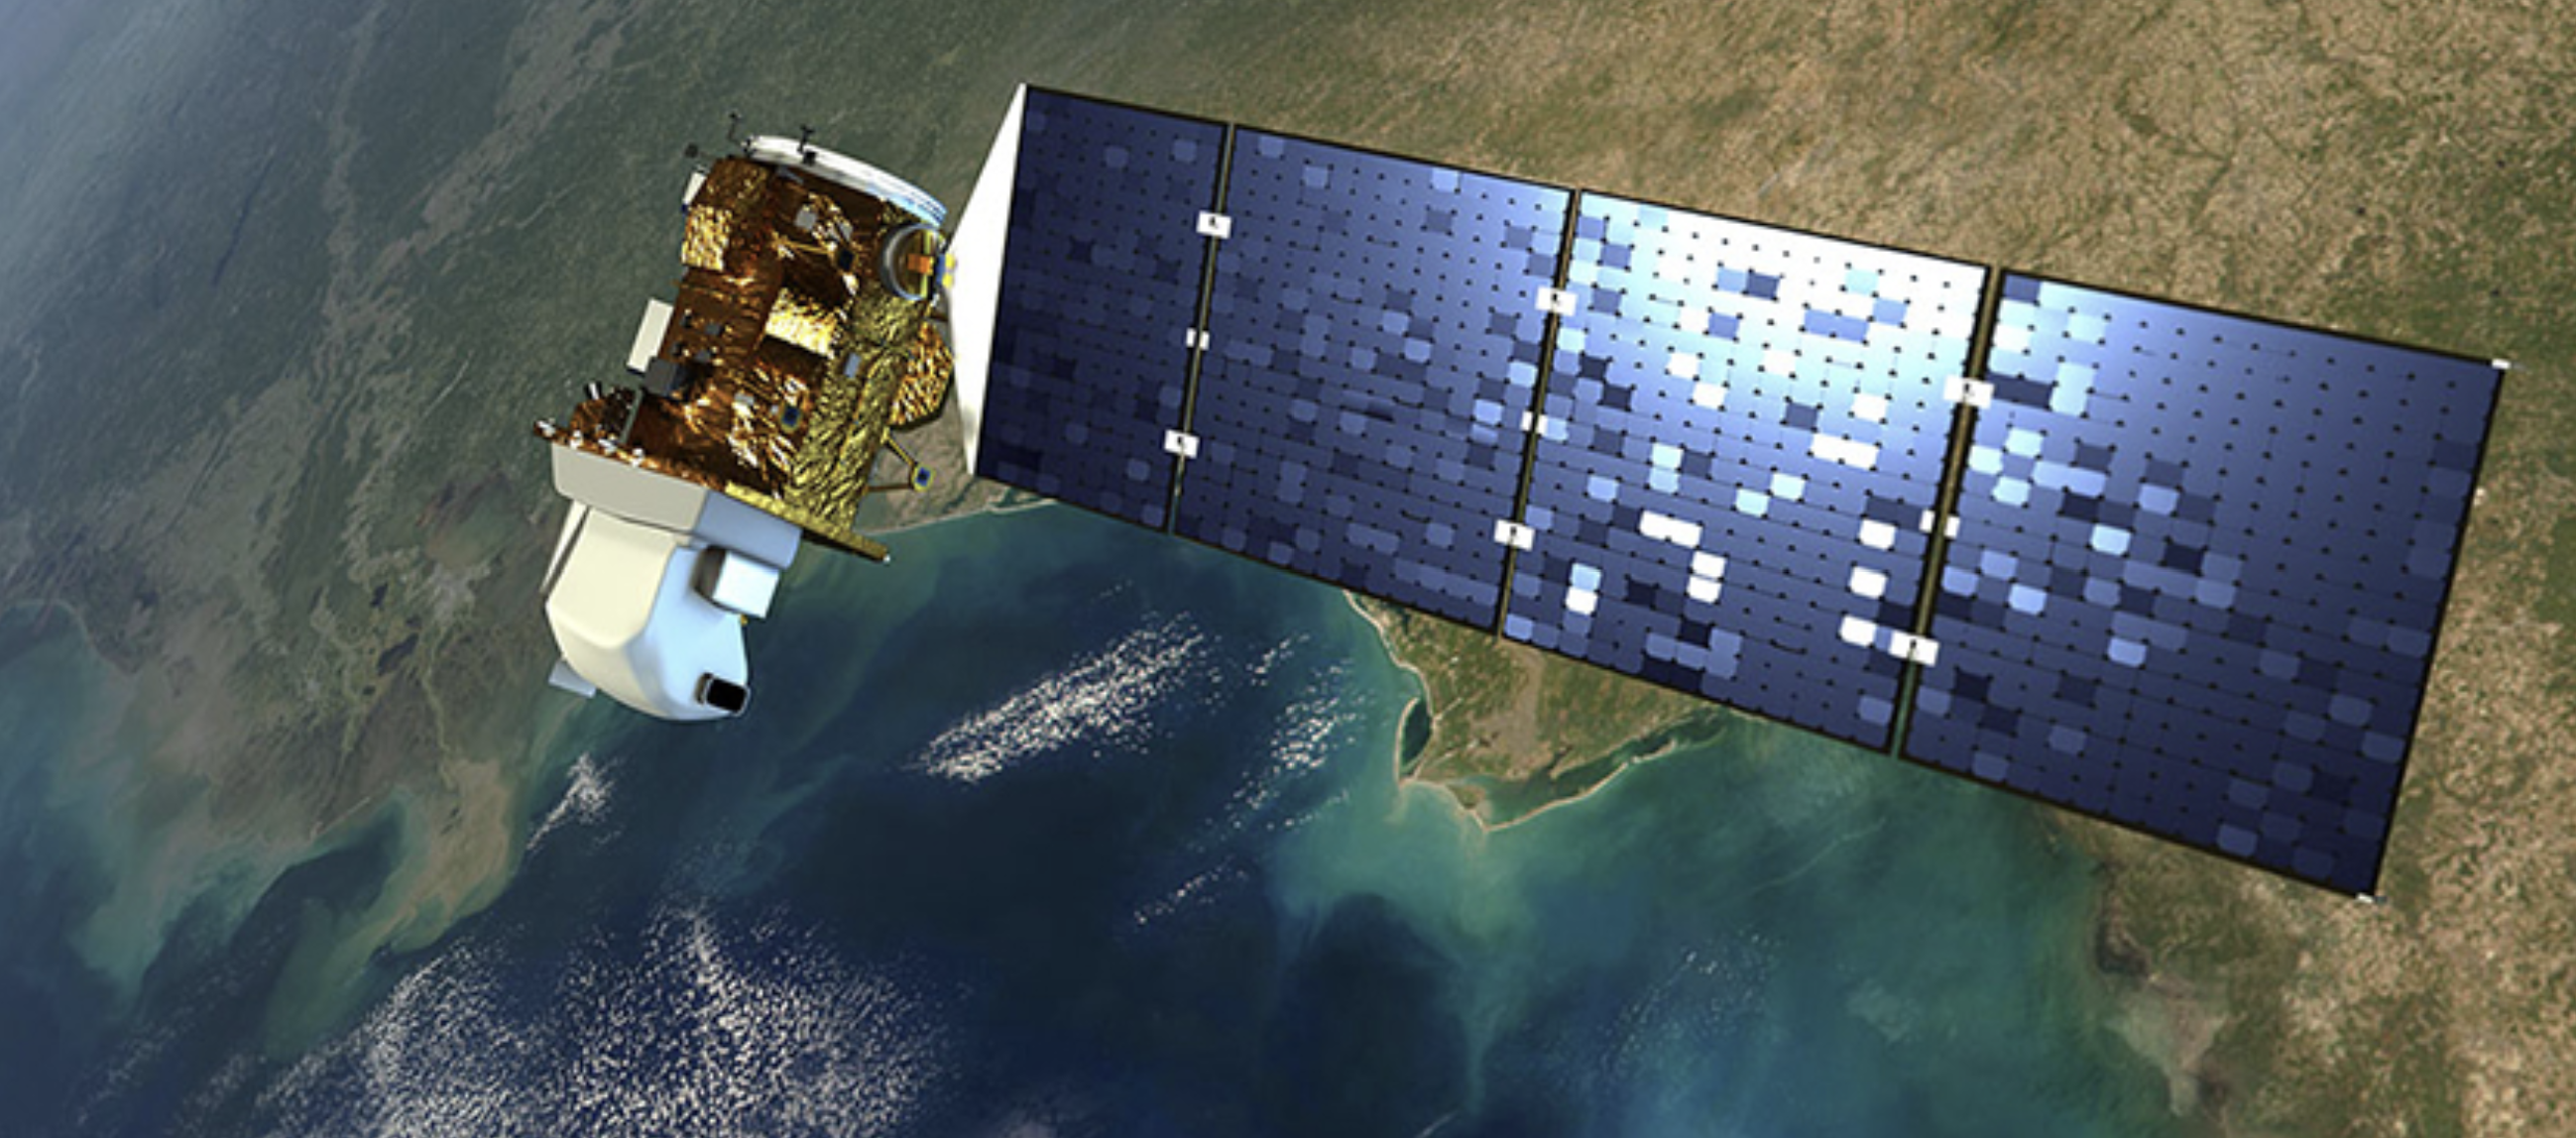
\includegraphics[width=4.1875in,height=\textheight]{images/clipboard-1188776161.png}

  }

  \caption{Copyright © NASA}

  \end{figure}
\item
  b. Sentinel 2A

  Sentinel 2 revisits the earth every 5 days (using both satellite A and
  B), meaning that it provides frequent observations and make it
  suitable to monitor rapid changes.
\end{itemize}

\begin{itemize}
\item
  \begin{figure}

  {\centering 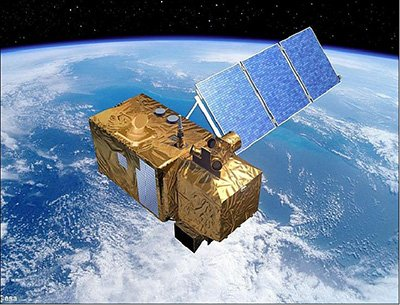
\includegraphics{images/clipboard-3938270325.png}

  }

  \caption{Copyright © ESA and AIRBUS Defence \& Space.}

  \end{figure}

  Each has their own characteristics, while Sentinel-2A has 10m spatial
  resolution Landsat-8 has 30m resolution. If we want to compare its
  spectral resolution we have to either upgrade or downgrade, usually
  downgrading the higher spatial resolution of Sentinel-2 (10m) to match
  Landsat's (30m) is the preferred approach.
\end{itemize}

\hypertarget{application}{%
\section{Application}\label{application}}

\textbf{In what ways can we use Sentinel and Landsat data?}

\begin{itemize}
\item
  Sentinel-2 (operated by ESA) has \emph{13 spectral bands} across a
  wide range of wavelengths, which are especially useful for vegetation
  monitoring, land cover classification, and agricultural applications.
\item
  Landsat 8 (operated by NASA and USGS) has \emph{11 spectral bands},
  which cover a similar range of wavelengths to Sentinel-2 but with
  fewer bands. Landsat 8 provides excellent coverage for land monitoring
  and vegetation studies as well.
\end{itemize}

They both could be used to vegetation monitoring, well\ldots\ldots..are
they really that difference?

\begin{itemize}
\item
  Sentinel-2 has more bands overall, with additional Red Edge bands, a
  higher spatial resolution (10m for key bands), and a Water Vapor band.
  This makes it more suited for \textbf{\emph{detailed vegetation
  analysis}}, agricultural monitoring, and atmospheric studies. In the
  paper\ldots..
\item
  Landsat 8, while having fewer bands, provides excellent coverage with
  a broader range of SWIR bands, and the addition of two thermal
  infrared bands makes it strong for land surface temperature and other
  \emph{\textbf{thermal analyses}.}
\end{itemize}

\textbf{Real world application of Sentinel and Landsat 8}

\begin{itemize}
\item
  \textbf{Landsat-8 application on detecting of vegetation evolution
  across China}

  This paper explores 30 years of landsat archive data (spaning of
  landsat 5 to 8) on 2.125 city to monitor the vegetation evolution. Han
  et al. (2025) use reflective bands such as Blue, green, red, NIR and
  SWIR (1 and 2) and highlighting vegetation characteristics using NDVI,
  EVI, and OSAVI. The NDVI and RGB bands were further processed to
  derive texture variables, including variance, contrast, entropy,
  angular second moment, and correlation. These texture metrics capture
  spatial patterns and fine-scale structural details of urban vegetation
  that may not be visible through spectral bands alone. I genuinely
  believe this finding has the potential to serve as a framework for
  evaluating the implementation of the government's long-term plan or
  the integration of policies across different administrations, which is
  often difficult to assess due to the extended time frame and
  transitions between ruling administrations.

  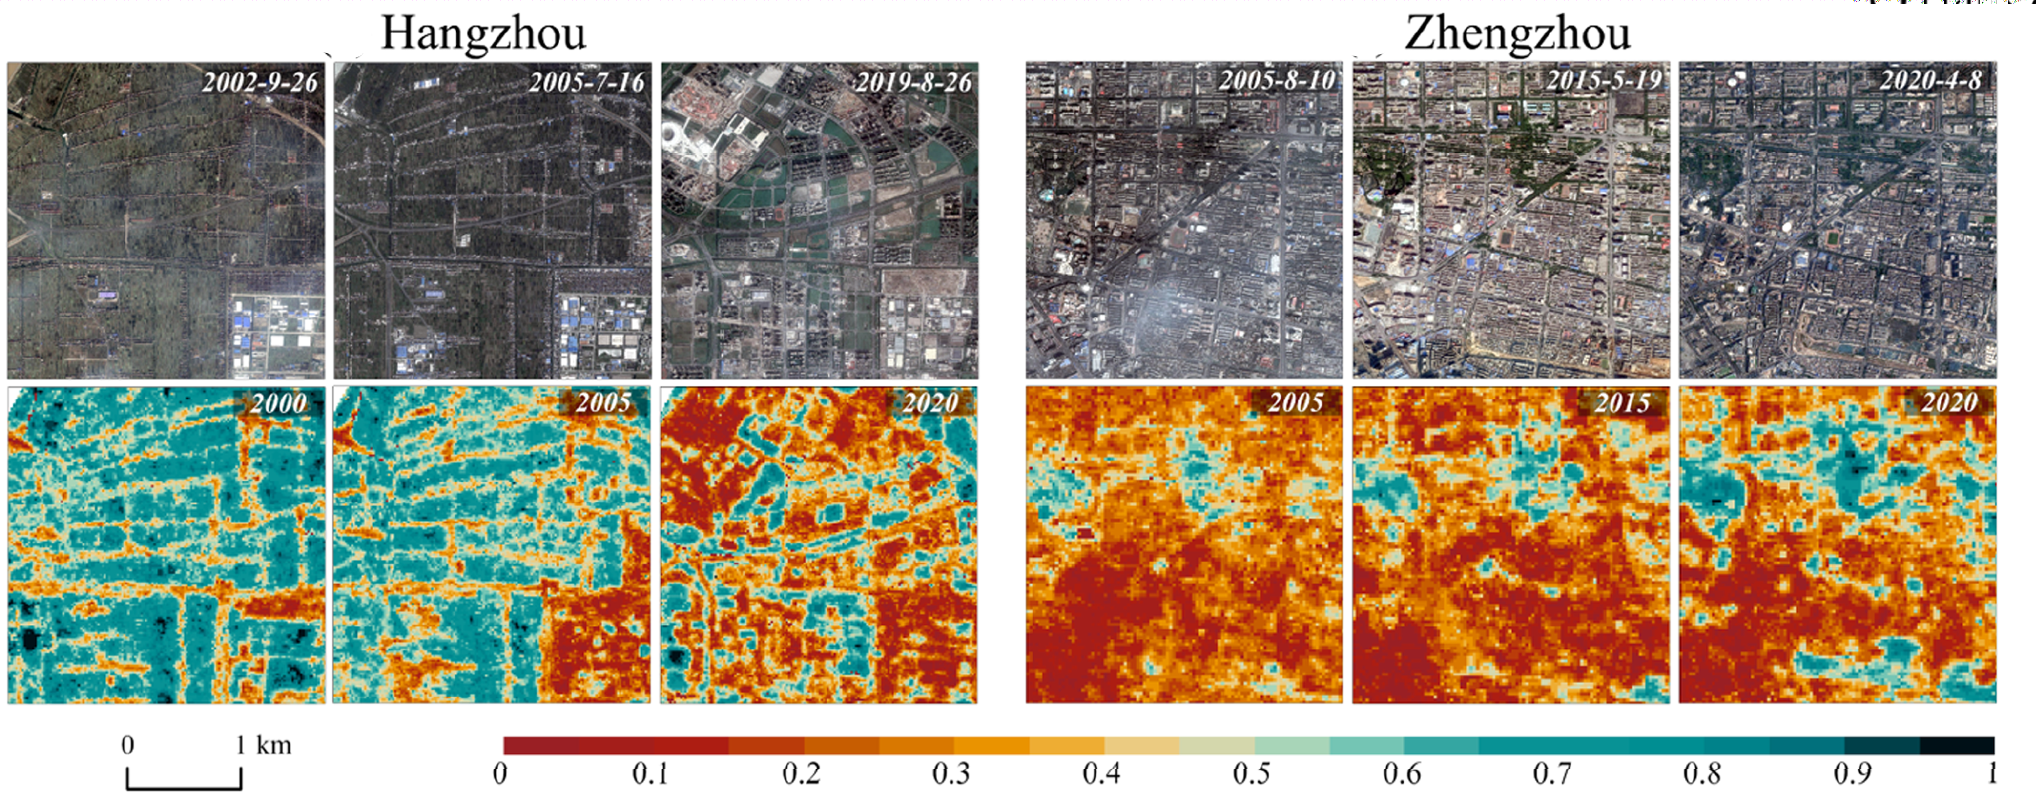
\includegraphics[width=6.96875in,height=\textheight]{images/clipboard-1072383063.png}

  Figure 1: A sample result shows urban vegetation degradation in
  Hangzhou and an increase in vegetation in Zhengzhou. source : (Han et
  al. 2025).
\item
  \textbf{Sentinel-2 application on plastic debris detecting on coastal
  area, Brazil}

  In this study, Nivedita et al. (2024) use 4 sensors of Sentinel Data
  to detect floating debris. After floating debris is detected they
  analyze spectral signature to differentiate trash by measuring the
  mean values of spectral signature of plastic and other materials (such
  as foam or seaweeds. This research, as part of monitoring marine
  pollution, could identify critical areas for conservation supports.

  \begin{figure}

  {\centering 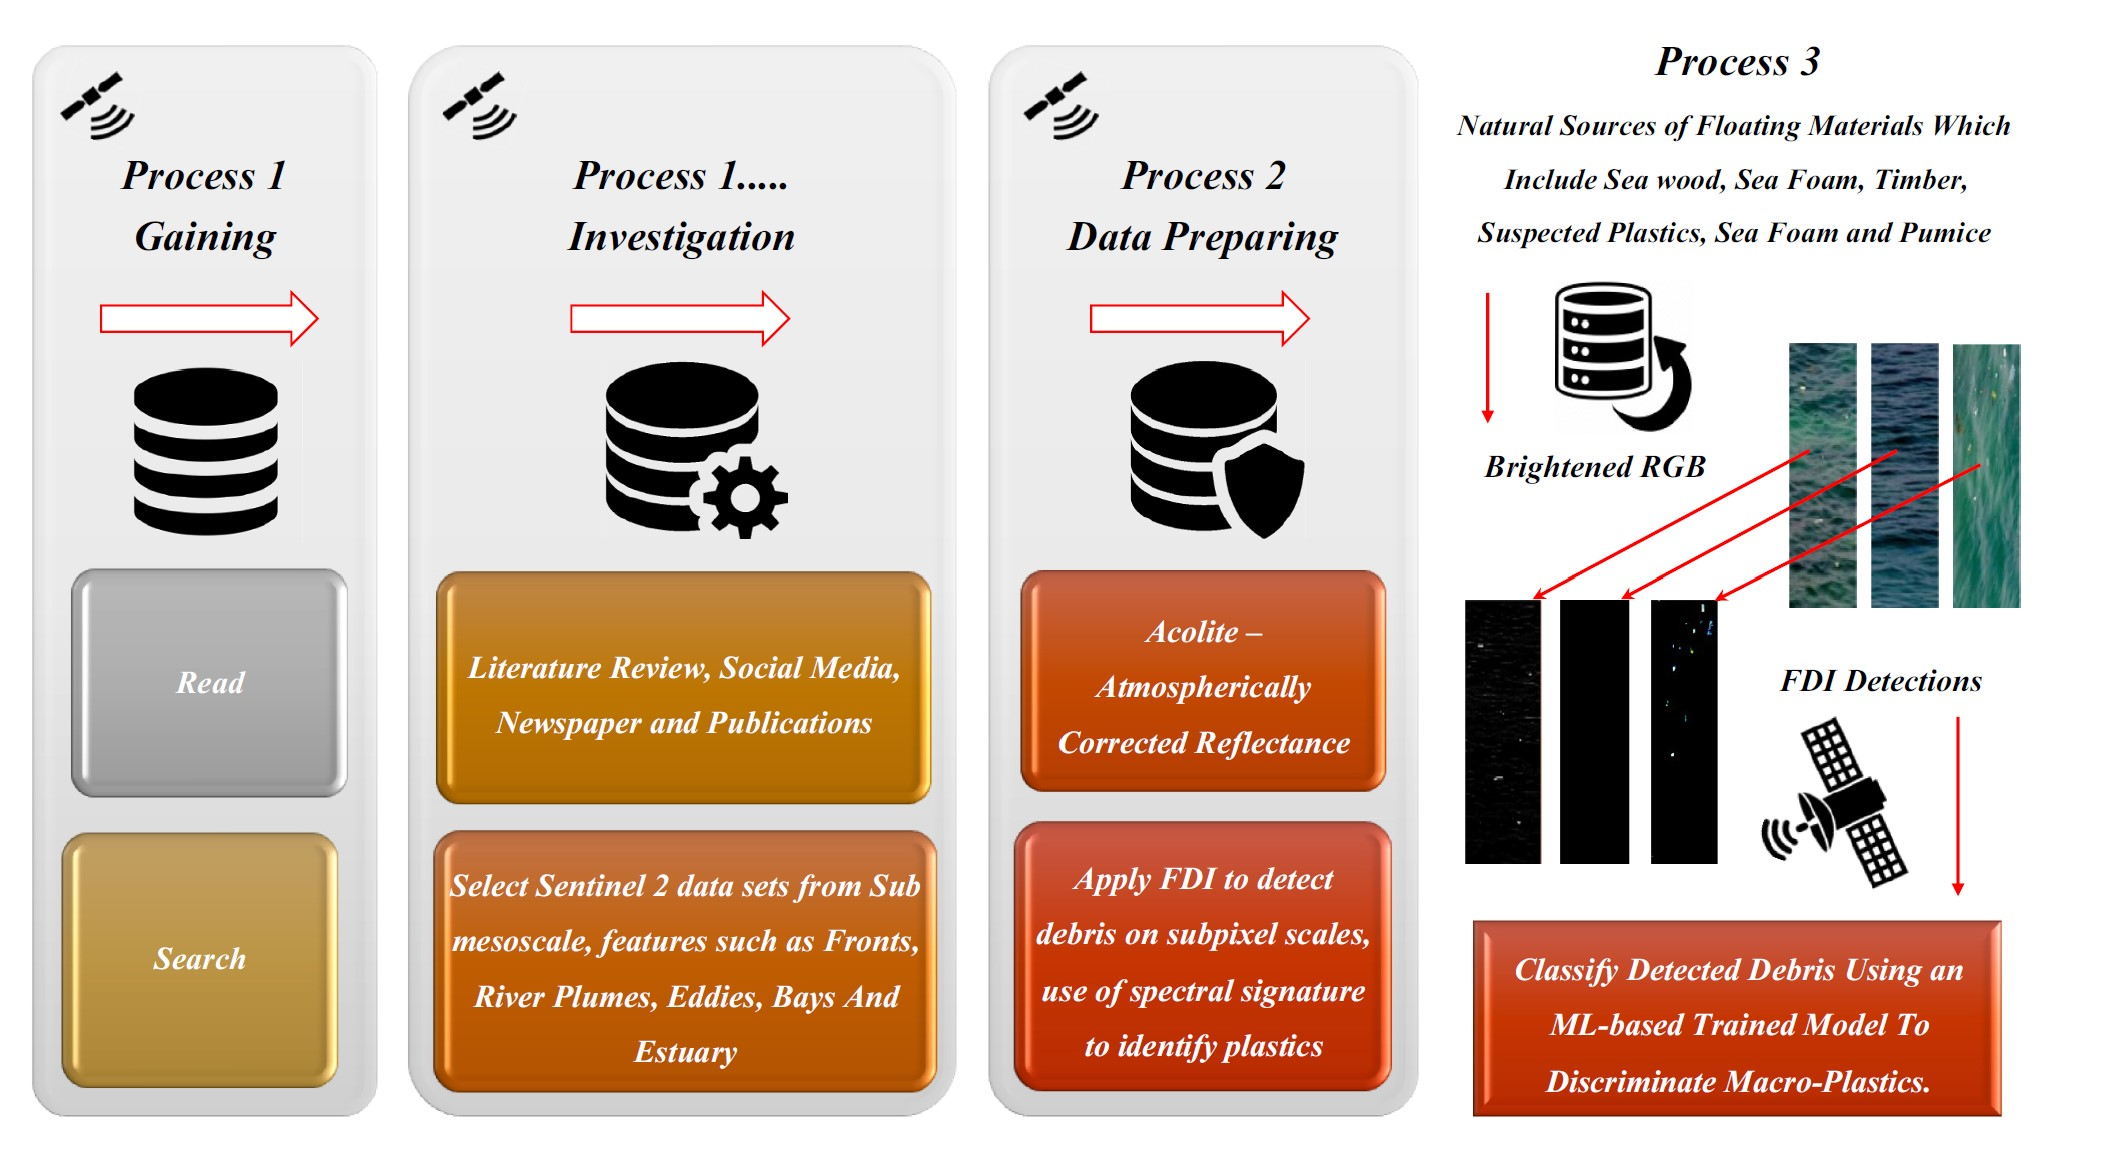
\includegraphics{images/Screenshot 2025-02-09 164424.jpg}

  }

  \caption{source :}

  \end{figure}

  Figure 2: Plastic Debris Detection. Source : (Nivedita et al. 2024)
\end{itemize}

\hypertarget{reflection}{%
\section{Reflection}\label{reflection}}

After exploring the application of the two selected satellites, I have
concluded that remote sensing data is particularly effective for
analyzing large-scale and long-term variations. It can also help
mitigate the high costs of manual data collection across vast regions.

This insight made me reflect on a similar challenge in my country,
Indonesia, the world's largest archipelago. The country needs to
identify which small islands are inhabited in order to provide essential
services to all of them. To address this, I'm considering using night
imagery data as a tool to distinguish inhabited islands from uninhabited
ones. The night time would indicate anthropogenic activities that are
associated~with~light at~night

\hypertarget{references}{%
\section{References}\label{references}}

\bookmarksetup{startatroot}

\hypertarget{xaringan-and-quarto-book}{%
\chapter{Xaringan and Quarto Book}\label{xaringan-and-quarto-book}}

Lecture this week reminded me of one of powerful figure in Uchiha Clan,
the one who can manipulate reality once he activates this-so-called
Xaringan. Well, but this Xaringan is not related to figures in Konoha's
world but related to a certain library in R Studio that enable us to
create neat HTML slides in R.

\hypertarget{summary-1}{%
\section{Summary}\label{summary-1}}

\begin{Shaded}
\begin{Highlighting}[]
\NormalTok{xaringanExtra}\SpecialCharTok{::}\FunctionTok{embed\_xaringan}\NormalTok{(}\AttributeTok{url =} \StringTok{"https://nooriza16.github.io/Xaringan/Xaringan.html"}\NormalTok{, }\AttributeTok{ratio =} \StringTok{"16:9"}\NormalTok{)}
\end{Highlighting}
\end{Shaded}

\hypertarget{reflections}{%
\section{Reflections}\label{reflections}}

For someone who is not familiar with html, learning Xaringan is
definitely challenging compared to powerpoint, as we just usually click
tabs on power point. Honestly, I still consider power point provides
more themes and more visualization effects that is easily to access
compared to Xaringan. However, as I delved further I realize that using
Xaringan is providing us with flexibility even such as positioned our
picture.

So far, I feel like Xaringan is best at incorporating snippet code on
presentation or interactive features that usually too heavy to load in
power point. Besides, it helps me to give a sense of what html look
like.

\bookmarksetup{startatroot}

\hypertarget{image-correction}{%
\chapter{Image Correction}\label{image-correction}}

\hypertarget{summary-2}{%
\section{Summary}\label{summary-2}}

\hypertarget{application-1}{%
\section{Application}\label{application-1}}

\hypertarget{reflections-1}{%
\section{Reflections}\label{reflections-1}}

I think performing Remote Sensing correction on R Studio is quite
challenging, as I become more used to using `button' in Remote Sensing
application such as ENVI or SNAP. Besides, after this week's lecture, I
genuinely think that Remote Sensing is quite complex as it is not only
an image but behind the imagery each pixel is composed by digital number
collection and it could be linked with regression too !

\bookmarksetup{startatroot}

\hypertarget{policy}{%
\chapter{Policy}\label{policy}}

\textbf{Project Case : A New Relocated Capital City of Indonesia ; From
Jakarta to Nusantara}

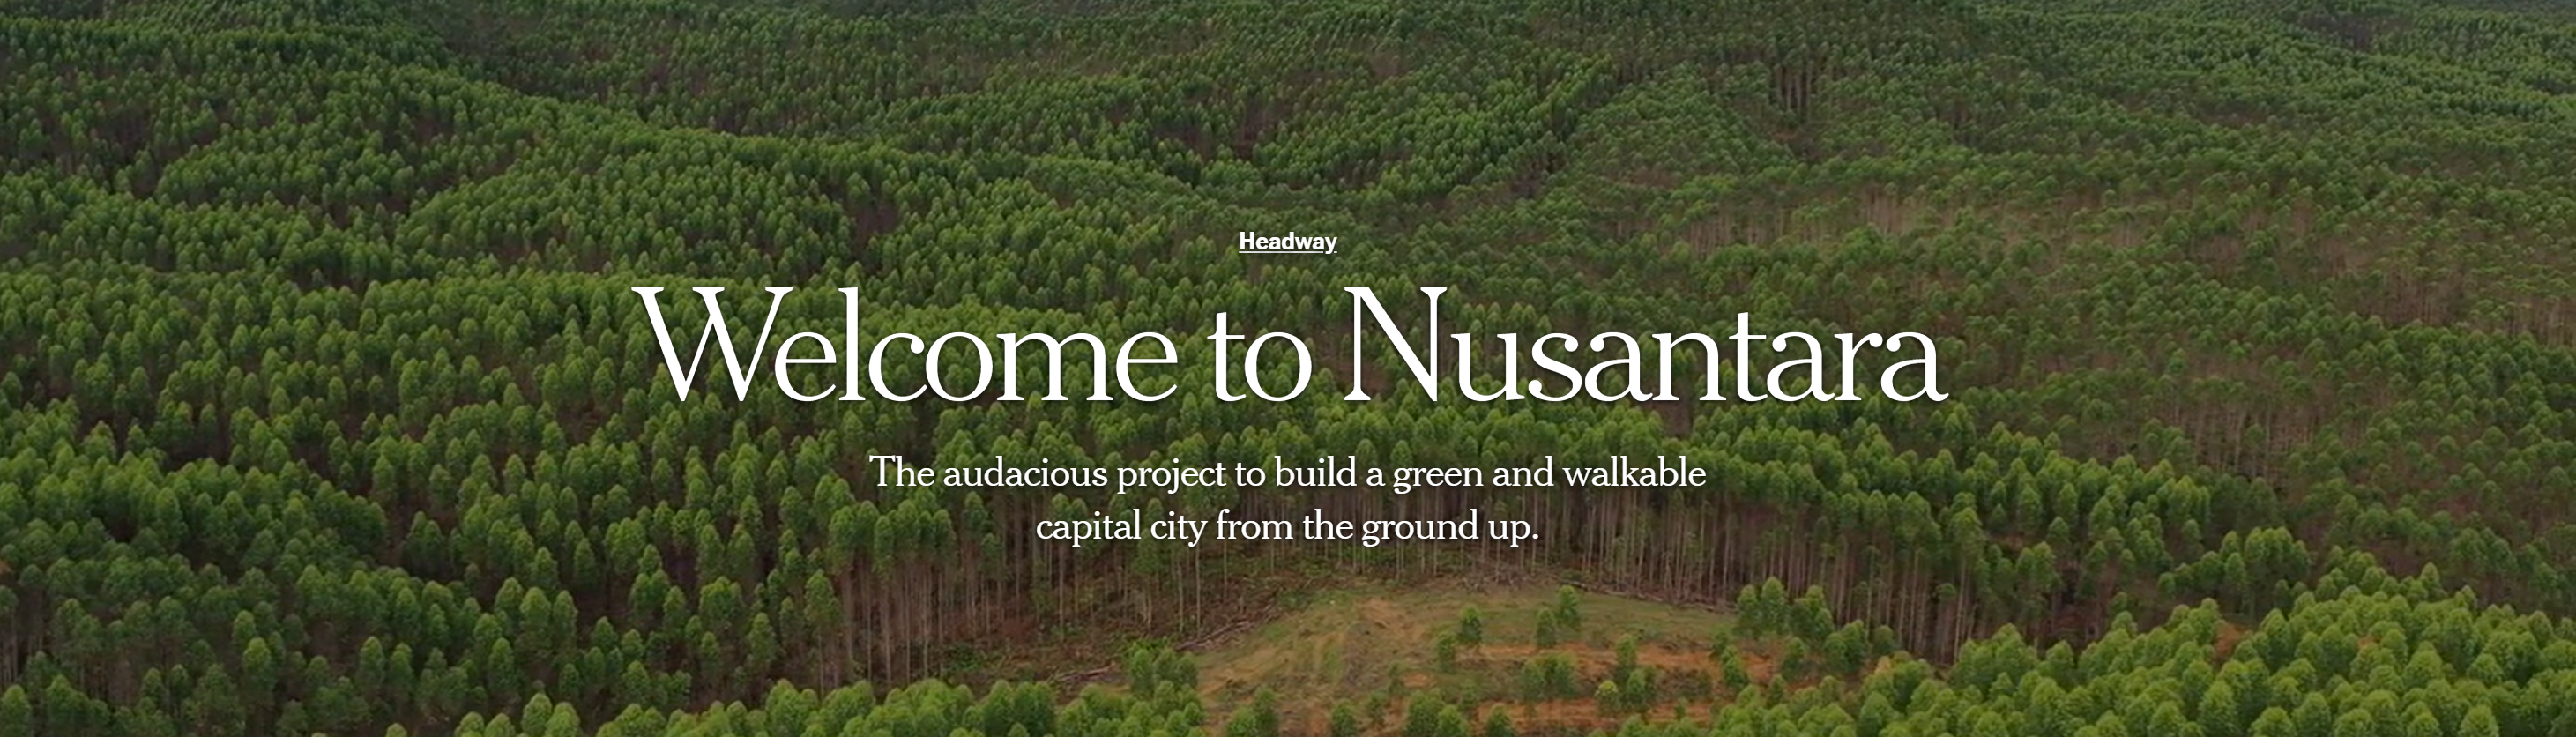
\includegraphics{images/clipboard-546673402.png}

Source :
\href{https://www.nytimes.com/interactive/2023/05/16/headway/indonesia-nusantara-jakarta.html}{www.nytimes.com}

\hypertarget{summary-3}{%
\section{Summary}\label{summary-3}}

Recently Indonesia planned to move its capital city from Jakarta (in
Java islands) into Penajam Paser Utara City (Borneo Islands), as the
current capital city, Jakarta, faced an issue of sinking, land
subsidence, overcrowding, low air and water quality (Bappenas 2021). The
term Nusantara is used to name this new capital city, symbolizing the
varied geographic settings and cultural diversities of Indonesia.

As for the time this published, Nusantara Development is on the phase 2
(2025-2029) that involved strengthening core area (housing, office,
commercial zone). Thus, in the time being, Jakarta will still remain the
capital of Indonesia until the Presidential Decree on the transfer of
the capital to Nusantara is issued. The issuance of this decree will
depend on the readiness of the new capital city, including the
preparation of all supporting systems such as infrastructure, human
resources, and governance systems.

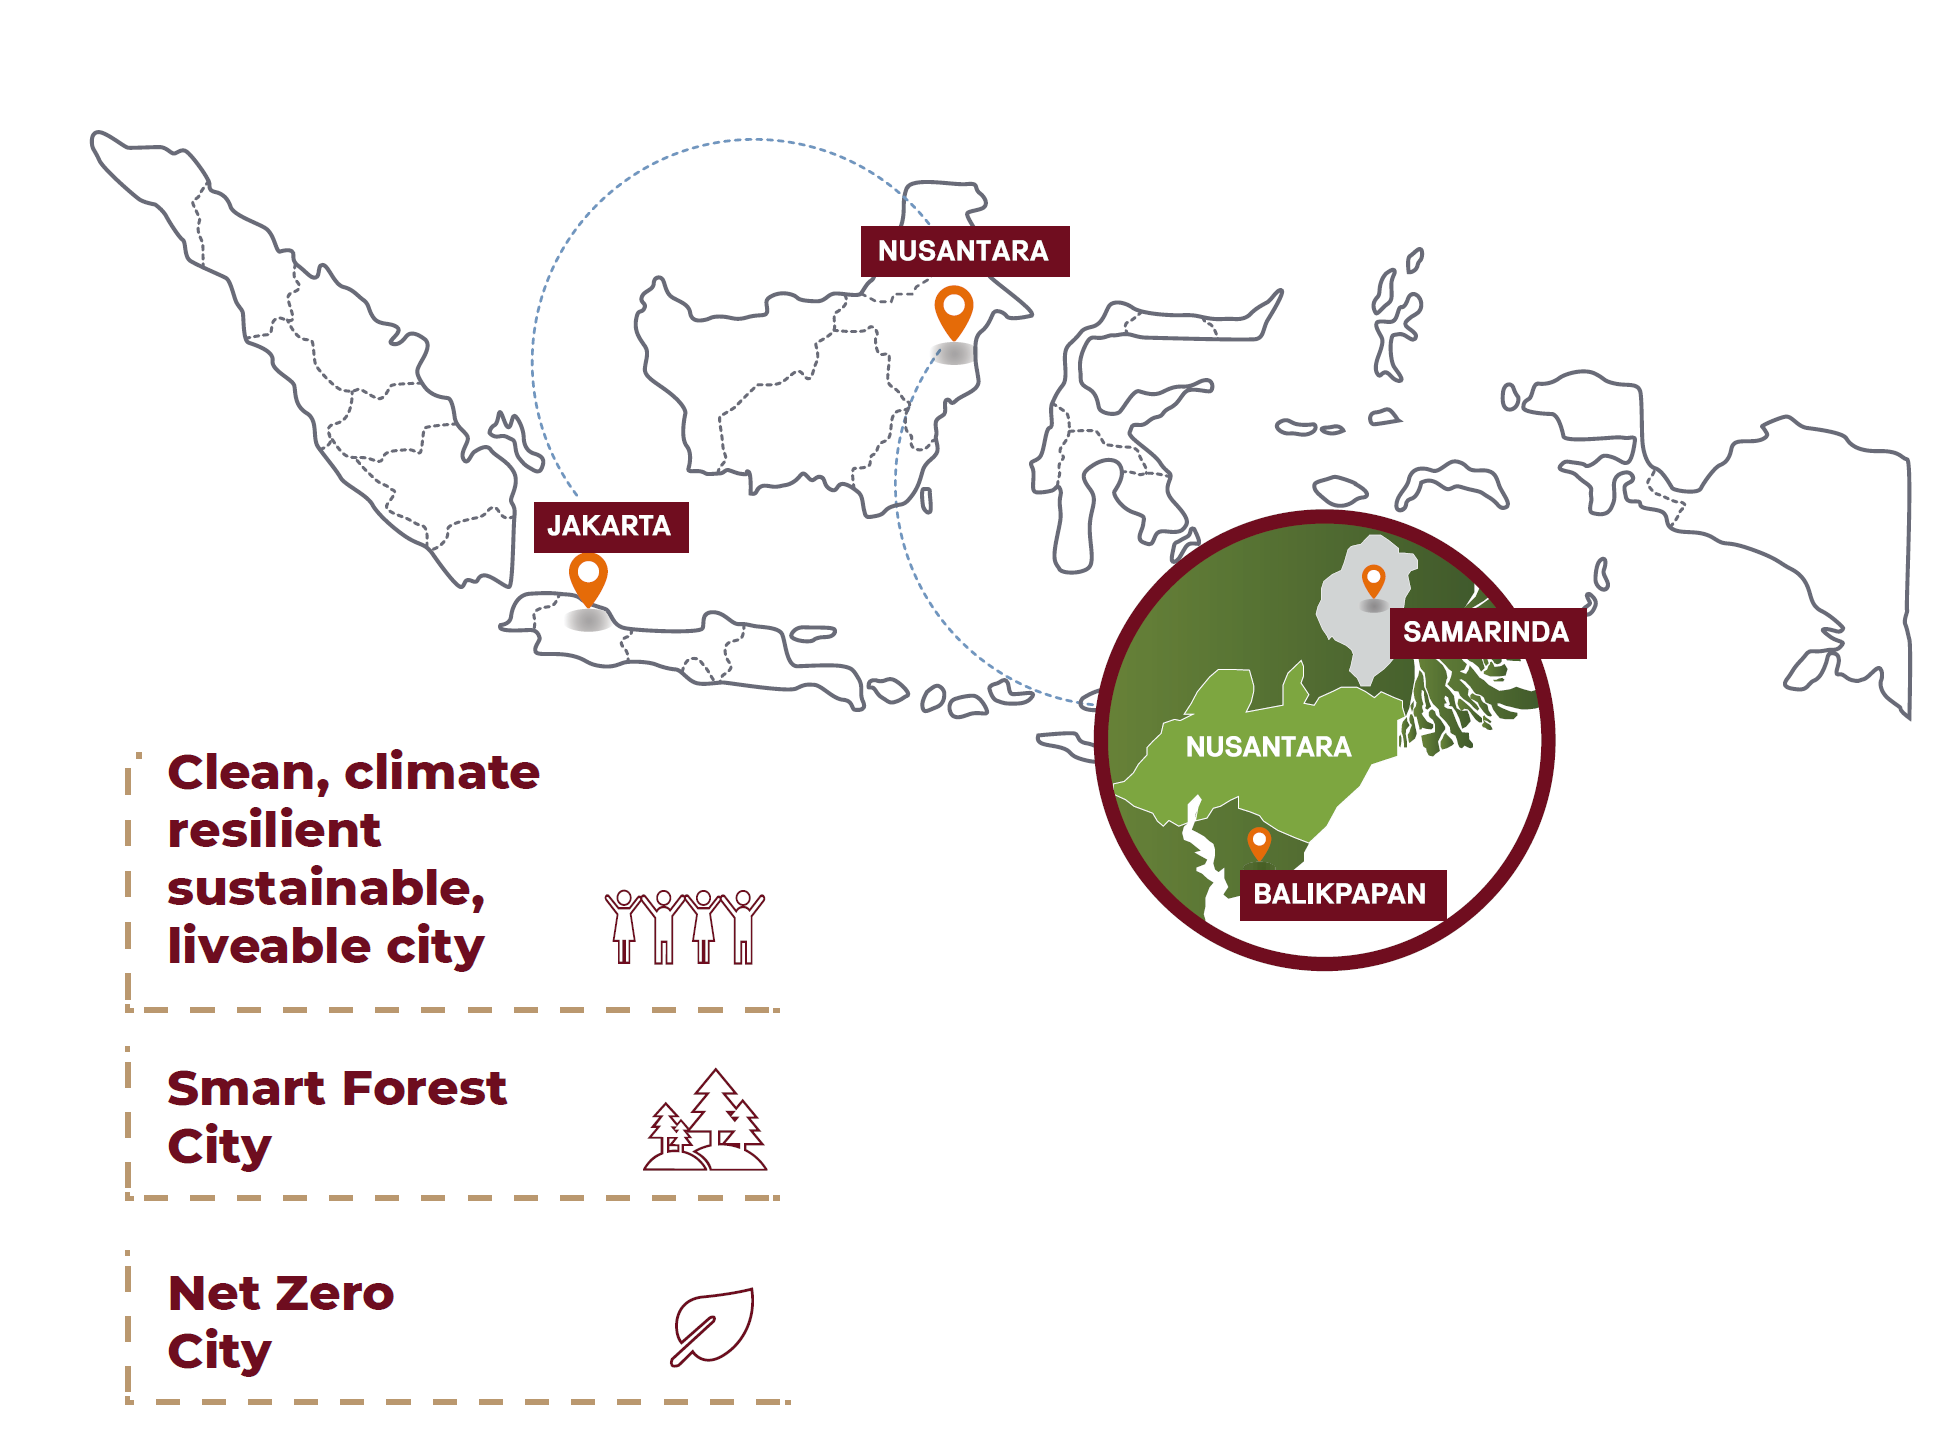
\includegraphics{images/clipboard-3462147358.png}

Figure 1: The Relocation Settings and Vision. source: (Capital Authority
2024)

As the development is still in the initial stage, the detailed planning
documents haven't been launched yet. Thus, I use available published
documents regarding the detail of Nusantara's Development which all of
them are publicly available, such as:

\begin{enumerate}
\def\labelenumi{\arabic{enumi}.}
\tightlist
\item
  \href{https://www.ikn.go.id/storage/pedoman-nusantara/2/nusantara-vlr-baseline-en.pdf}{Nusantara
  Sustainable Development Goals (SDGs) Voluntary Local Review Baseline
  {[}2024{]}}
\item
  \href{https://ikn.go.id/storage/pedoman-nusantara/1/nusantara-biodiversity-management-master-plan-2024.pdf}{Nusantara
  Biodiversity Management Master Plan} {[}2024{]}
\end{enumerate}

\begin{quote}
\textbf{Policy}
\end{quote}

The new capital city, Nusantara, is designed as a \textbf{forest city},
with 75\% of its designated area being green space. This design aims to
create a harmonious blend of urban development and biodiversity hotspots
(Borneo Island, where Nusantara is located, is famous for its tropical
rainforests). However, the design of being a forest city, its proximity
to the rainforest, and its drive on landscape change would present
significant \textbf{challenges}. One of the major concerns is the
increasing likelihood of mosquito-borne diseases (such as
\textbf{malaria}) spreading in the new capital, which are prevalent in
tropical regions Surendra et al. (2024).

Addressing this risk is essential, as Nusantara aims to become a
sustainable city aligned with the Sustainable Development Goals (SDGs).
However, there is currently no official framework from the government
for mitigating malaria risk in Nusantara, as the primary focus remains
on infrastructure development. Since malaria is both a global and local
challenge, certain goals should be considered to support Nusantara's
sustainability, such as:

\textbf{A. Global Goals :} Sustainable Development Goals (SDGs) 3.3 :
Fight Communicable Diseases

The SDGs propose achievable global in combating malaria with target that
in include reducing incident, mortality rates, eliminate malaria in 35
countries by 2030 and prevent resurgence of the disease in a
malaria-free country. Meanwhile, Indonesia's estimated malaria incidence
per 1000 population at risk is still on range between 1-50 incidents per
1000 population in 2023.

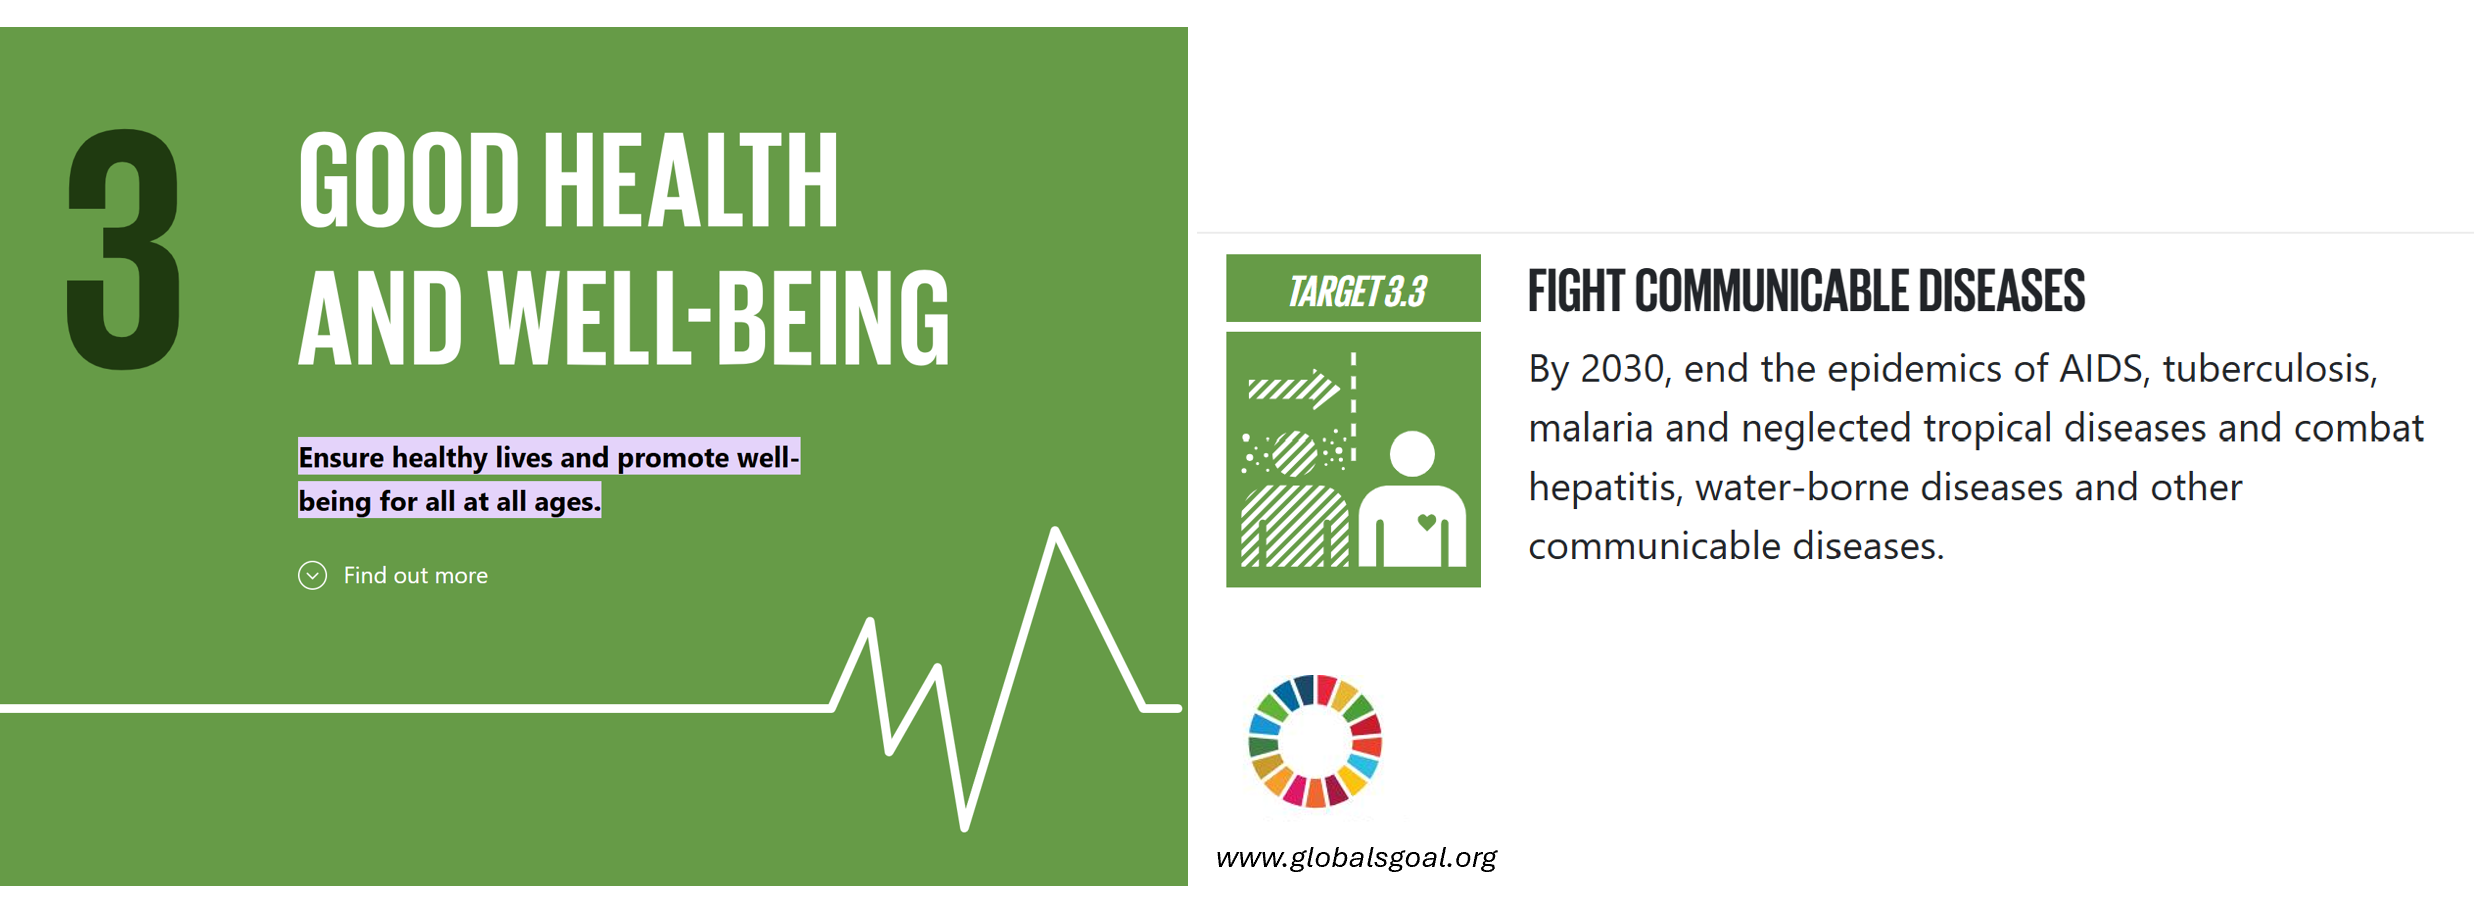
\includegraphics{images/clipboard-3146823061.png}

Figure 2 : SDGs Goal related to Malaria. source : globalsgoal.org

To achieve the Global Goals, WHO launched global technical strategy for
malaria 2016-2030 with frameworks such as:

\begin{itemize}
\item
  Pillar 1 : Ensure access to malaria prevention, diagnosis and
  treatment as part of universal health coverage.

  Keywords I underlined in this pillar is : Countries should collect
  \textbf{data} across all settings, including those areas that are
  malaria-free but at risk of re-establishment of malaria .
\item
  Pillar~3. Transform malaria surveillance into a key intervention.

  Keywords I underlined in this pillar is : surveillance in areas of
  high \& low transmission and in areas targeted for elimination
\end{itemize}

\textbf{B. Local Goals :} Eliminate malaria case by 2030 and maintain
malaria free status

Translating the global goals on malaria elimination, Indonesia's
Ministry of Health (Ministry of Health and Control 2023) had proposed
recommendations, including the new capital city such as:

\begin{itemize}
\item
  Malaria elimination policies and implementation need basic research,
  operational support, and efficient technology development.
\item
  Provide input to the IKN special authority regarding malaria risk to
  ensure the design of the IKN area drainage system is free from malaria
  mosquito larvae habitat
\item
  Mapping legal and illegal forest encroachers to develop an activity
  plan and budget
\end{itemize}

\hypertarget{application-2}{%
\section{Application}\label{application-2}}

\begin{quote}
Remote Sensing as Baseline for detecting malaria hotspot
\end{quote}

In malaria elimination, remote sensing could be beneficial as a baseline
data for mapping malaria hotspot by incorporating climatic factors and
landuse factors to detect mosquito habitat as what (Wimberly et al.
2021) aggregated in framework on Figure 1. Dataset for the Nusantara
analysis could use imagery product which is able to highlight water
bodies and wetland (proxy for breeding sites), vegetation and land cover
(proxy for mosquito habitat), surface temperature (proxy for mosquito
activity), and topography (potential inundation area). We could use
rainfall season for in our dataset, however If we have yearly rainfall
data perhaps we could identify the pattern of rainfall session to get
more informed when picking the time series.

Earth observation data commonly used in malaria research included
Sentinel-2 and Landsat 8, although Sentinel-2 is preferred because its
finer resolution and its frequent visit. However, (Wimberly et al. 2021)
mentioned that those resolution is still too coarse to detect individual
larva habitat and breeding thus suggest Very High Resolution imagery
(such as Pleaides, WorldView) or SAR imagery (such as C-band SAR
Sentinel-1 data) that able to penetrate cloud cover during the wet
season.

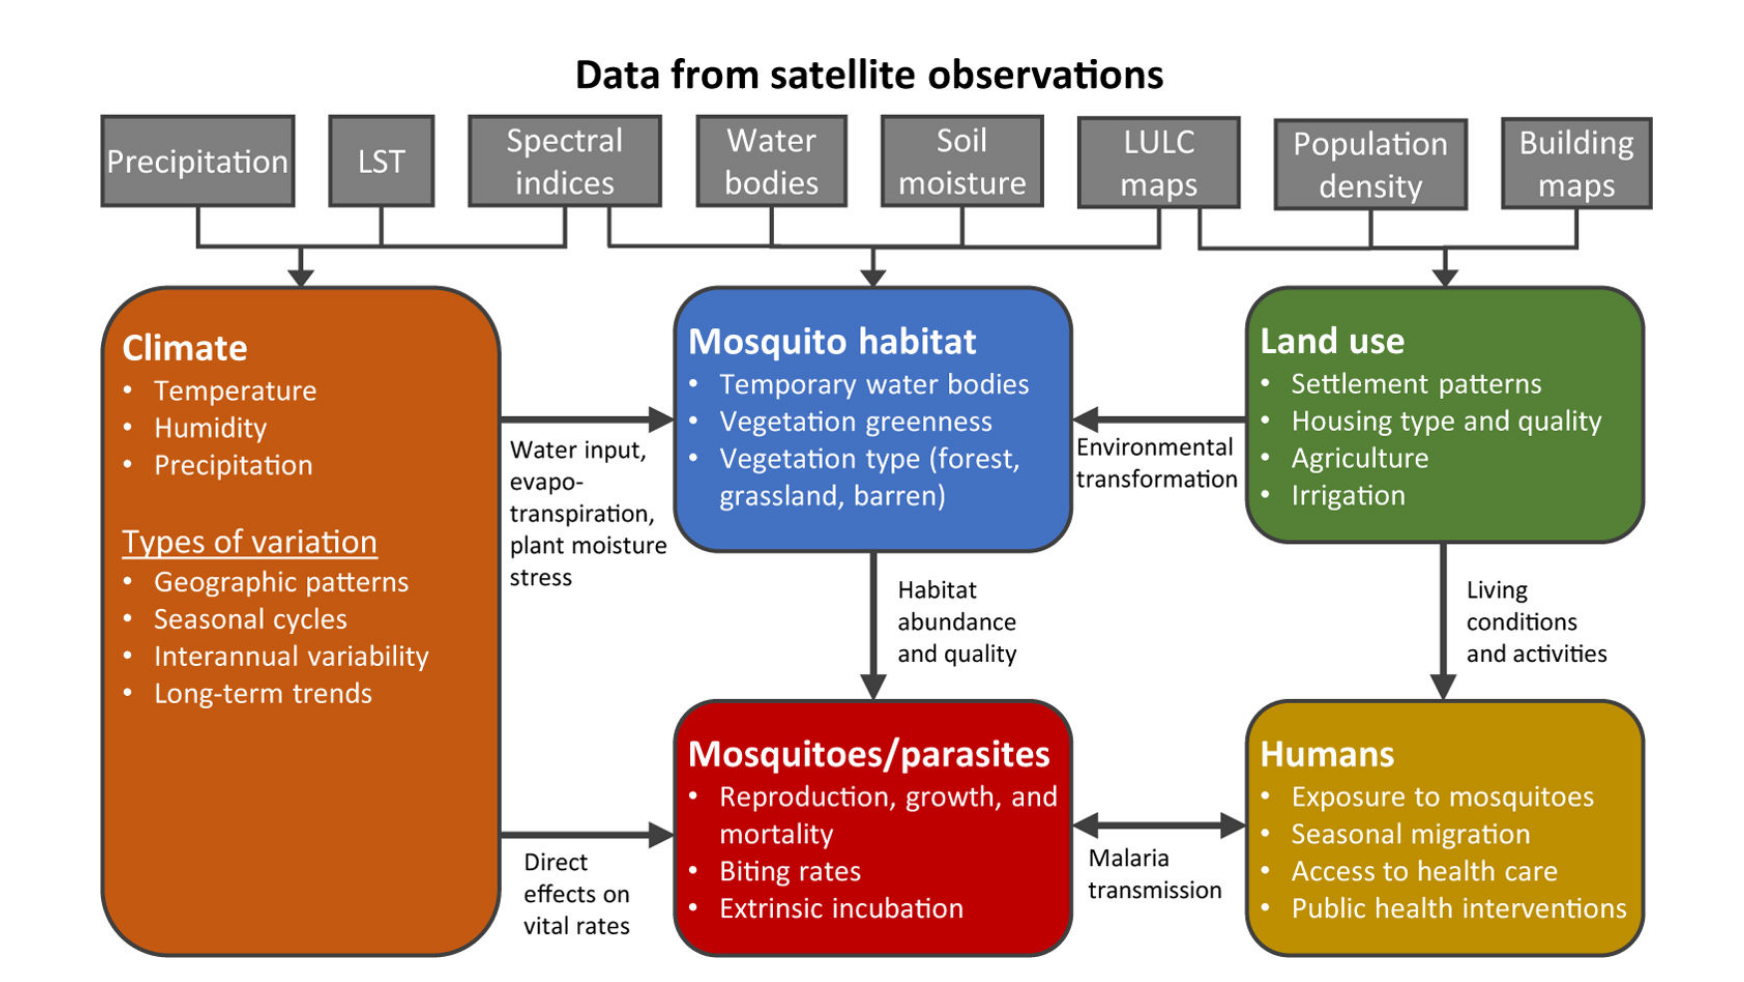
\includegraphics{images/clipboard-687725868.png}

Figure 2: Framework in which Remote Sensing used in Malaria studies.
source : Wimberly et al. (2021).

\hypertarget{reflections-2}{%
\section{Reflections}\label{reflections-2}}

During this week, I got a lot of reflections on my mind because I
finally found lecture that explicitly bridging the gap of `academics' to
real-world policy. One the most important key-takeaway from the lecture
is that ``some academics papers are too technical, without clearly
addressed policy; some policy don't include academic findings they could
benefit for''.

My reflections would be:

\begin{quote}
\begin{enumerate}
\def\labelenumi{\arabic{enumi}.}
\tightlist
\item
  Remote Sensing is good, but combining with GIS is better
\end{enumerate}
\end{quote}

From the result in step 1, we could then investigate the result using
the malaria incident data to validate our classification result, what
percentage of areas classified as high risk have recorded incidents, and
which areas have not? As I delved further into the framework in
eliminating Malaria both Global and Local framework, they have mentioned
to aggregate data about the incidents, high risk, low risk but not
explicitly mentioned using map. With map, we could easily overlay this
hotspot with malaria incidents, landuse, and potentially social-economic
data as

\begin{quote}
\begin{enumerate}
\def\labelenumi{\arabic{enumi}.}
\setcounter{enumi}{1}
\tightlist
\item
  Remote Sensing and GIS is good, but interpreting the data with
  affected communities is better
\end{enumerate}
\end{quote}

Aside from remote sensing data, I would like to combine the analysis by
incorporating local wisdom in responding to Malaria. This approach would
enhance the understanding of how to mitigate this issues, as these
communities have lived for a long time near the rainforest and are
directly affected.

\begin{quote}
\begin{enumerate}
\def\labelenumi{\arabic{enumi}.}
\setcounter{enumi}{2}
\tightlist
\item
  Challenges of implementation, collaboration is a key
\end{enumerate}
\end{quote}

I resonate a lot with the lecture's key takeaway as I genuinely think
academics and urban governance still have a distance between them. In
terms of human resources, that make the adoption of academics finding
hard to implement in governments. Besides, government project is based
on annual budget which is make it a fast-paced environment that need an
immediate output which make them reluctant to go through experimental
phase often found in academics processes. Thus collaboration is a key
between

\hypertarget{references-1}{%
\section*{References}\label{references-1}}
\addcontentsline{toc}{section}{References}

\hypertarget{refs}{}
\begin{CSLReferences}{1}{0}
\leavevmode\vadjust pre{\hypertarget{ref-bappenas2021}{}}%
Bappenas, Kementrian PPN. 2021. {``Buku Saku Pemindahan Ibu Kota
Negara.''}

\leavevmode\vadjust pre{\hypertarget{ref-capitalauthority2024}{}}%
Capital Authority, Nusantara. 2024. {``Nusantara Sustainable Development
GOals (SDGs) Voluntary Local Review Baseline.''}

\leavevmode\vadjust pre{\hypertarget{ref-han2025}{}}%
Han, Yuan, Jianhua He, Xiaoping Du, Xiao Han, and Yaolin Liu. 2025.
{``Reconstructing Urban Vegetation Evolution in China Using Multimodal
Deep Learning and 30-Years Landsat Archive.''} \emph{Urban Forestry \&
Urban Greening} 103 (January): 128582.
\url{https://doi.org/10.1016/j.ufug.2024.128582}.

\leavevmode\vadjust pre{\hypertarget{ref-ministryofhealth2023}{}}%
Ministry of Health, Directorate General of Disease Prevention, and
Control. 2023. {``National Action Plan for Acceleration of Malaria
Elimination 2020-2026 (Revision).''}
\url{https://malaria.kemkes.go.id/sites/default/files/2024-08/National\%20Strategic\%20Plan\%20Revision_Malaria_29\%20Mei\%202023.pdf}.

\leavevmode\vadjust pre{\hypertarget{ref-nivedita2024}{}}%
Nivedita, V., S. Sabarunisha Begum, Ghadah Aldehim, Abdullah M.
Alashjaee, Munya A. Arasi, Mohamed Yacin Sikkandar, T. Jayasankar, and
S. Vivek. 2024. {``Plastic Debris Detection Along Coastal Waters Using
Sentinel-2 Satellite Data and Machine Learning Techniques.''}
\emph{Marine Pollution Bulletin} 209 (December): 117106.
\url{https://doi.org/10.1016/j.marpolbul.2024.117106}.

\leavevmode\vadjust pre{\hypertarget{ref-surendra2024}{}}%
Surendra, Henry, Bimandra A. Djaafara, Helen D. Prameswari, Dedy
Supriyanto, Ponco Waluyo, Setyo B. Basuki, Herdiana Herdiana, et al.
2024. {``Mitigating Risks of Malaria and Other Vector-Borne Diseases in
the New Capital City of Indonesia.''} \emph{Nature Communications} 15
(1): 10575. \url{https://doi.org/10.1038/s41467-024-54891-x}.

\leavevmode\vadjust pre{\hypertarget{ref-wimberly2021}{}}%
Wimberly, Michael C., Kirsten M. de Beurs, Tatiana V. Loboda, and
William K. Pan. 2021. {``Satellite Observations and Malaria: New
Opportunities for Research and Applications.''} \emph{Trends in
Parasitology} 37 (6): 525--37.
\url{https://doi.org/10.1016/j.pt.2021.03.003}.

\end{CSLReferences}



\end{document}
